\documentclass[10pt,a4paper]{article}
\textheight245mm
\textwidth170mm
\hoffset-21mm
\voffset-15mm
\parindent0pt
\usepackage[utf8]{inputenc}
\usepackage{amsmath,amsfonts,amssymb}
\usepackage{dsfont}
\usepackage{graphicx}
\usepackage{caption}

\begin{document}
\title{TIPE : Matrices aléatoires et théorème de Wigner}
\date{2021-2022}
\author{Sacha BEN-AROUS}
\maketitle 
\section{Introduction}

L'objectif de ce document est d'établir une version simple du théorème de Wigner, aussi appelé loi du demi-cercle. Celui-ci décrit l'évolution des valeurs propres de matrices symétriques dont les entrées sont des variables aléatoires indépendantes, identiquement distribuées (noté i.i.d dans la suite) et centrées. Sous une 'bonne' normalisation, l'histogramme des valeurs propres tend alors vers un demi-cercle de rayon 2, de centre 0. L'un des intérêts de ce théorème est son caractère universel : peu importe la loi des entrées, le spectre normalisé tendra toujours vers le demi-cercle.

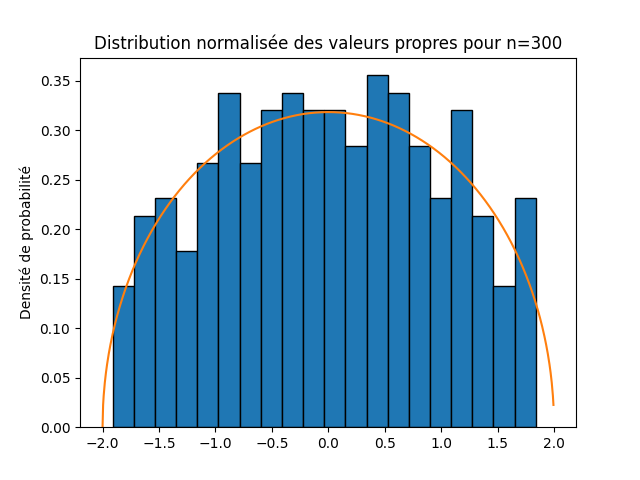
\includegraphics[scale=0.452]{Figure_300.png} 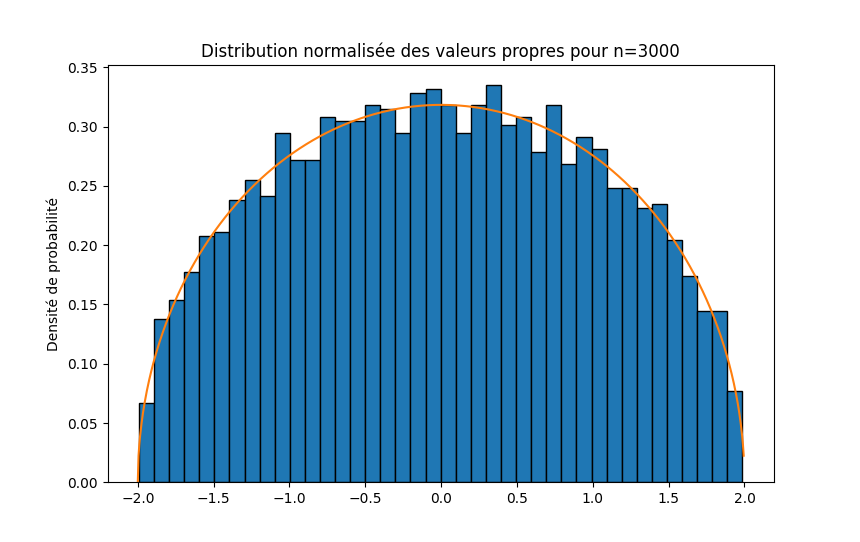
\includegraphics[scale=0.4]{Figure_1.png}
\captionof{figure}{Exemple dans le cas d'entrées suivant une loi de Rademacher}


\section{Présentation du problème}
	On se donne une suite de  variables aléatoires symétriques i.i.d $(W_{i,j})_{i,j \in \mathbb{N}} $ qui vérifie : $\mathbb{E}(W_{1,1})=0 $, $ \mathbb{E}\left (\left| W_{1,1}  \right|^2\right )=1 $  et  $ \forall k \geq 3 $, $ \mathbb{E}(\left| W_{1,1}  \right|^k) < +\infty $ . On note $W_n := (W_{i,j})_{1 \leq i,j \leq n}$ et $\text{SP}(\frac{W_n}{\sqrt{n}})= \{ \lambda_i , i \in \{1,\dots,n\}\} $.\\
L'énoncé que l'on se propose de démontrer est le suivant : \\


\textbf{Théorème (Wigner):} \textit{Pour toute fonction $f$ continue bornée : 
\[ \lim_{n \to \infty} \mathbb{E}\left (\frac{1}{n} \sum_{i=1}^n f(\lambda_i)\right ) = \int_{-2}^2 f(x) \, \mathrm{d}\mu_{SC} \] où $\mathrm{d}\mu_{SC}$ est la densité du demi-cercle de rayon 2, de centre 0, définie par : \[\mathrm{d}\mu_{SC}(x) =\frac{1}{2\pi}\mathds{1}_{[-2;2]}(x)\sqrt{4-x^2} \mathrm{d}x\] }\\

\textbf{Remarque :} Si plus généralement $ \mathbb{E}(\left| W_{1,1}  \right|^2)= \sigma^2 $, le demi-cercle limite est alors de rayon $2\sigma$, de densité : $\mathrm{d}\mu_{SC}^{(\sigma)}(x) =\frac{1}{2\pi{\sigma^2}}\mathds{1}_{[-2;2]}(x)\sqrt{4\sigma^2-x^2} \mathrm{d}x$ \\

\textbf{Remarque :} Une façon de voir le lien entre le théorème précédent et le commentaire en introduction sur l'histogramme des valeurs propres normalisées est, en admettant que l'on puisse le faire, d'appliquer le théorème précédent avec $f$ la fonction indicatrice du segment $[-\infty;a]$, où $a \in [-2;2]$ : on a 
\[\lim_{n \to \infty} \mathbb{E}\left (\frac{1}{n} \sum_{i=1}^n \mathds{1}_{[-\infty;a]}(\lambda_i)\right ) = \int_{-2}^2 \mathds{1}_{[-\infty;a]}(x) \, \mathrm{d}\mu_{SC} \]
Soit \[\lim_{n \to \infty} \mathbb{E}\left (\frac{|\{i, \lambda_i \leq a \}|}{n}\right )=\int_{-\infty}^a \mathrm{d}\mu_{SC}\]
Ainsi, à la limite, la densité des $(\lambda_i)_{i \in \mathbb{N}}$ est donnée par la densité du demi-cercle.
\\

\textbf{Plan}

La démonstration se déroulera en trois étapes : 
\begin{enumerate}
	\item La démonstration du théorème 1.1 dans le cadre des monômes $(X^k)_{k \in \mathbb{N}}$
	\item L'extension aux fonctions continues à support compact via le théorème de Weierstrass.
	\item L'obtention du cas général grâce à une borne sur la valeur propre maximale.
\end{enumerate}

\section{Nombres de Catalan}

Les calculs des sections suivantes vont faire apparaître les nombres dits "de Catalan" par le biais du dénombrement d'ensembles bien choisis. On va donc montrer quelques propriétés vérifiées par ces nombres :\\

\textbf{Définition (Catalan):} \textit{ On note : $\forall n \in \mathbb{N}$, $Cat(n)=\frac{(2n)!}{(n+1)!n!}$ }\\

\textbf{Lemme 3.1 :}\textit{ $(Cat(n))_{n \in \mathbb{N}}$ est l'unique suite vérifiant : $\begin{cases} u_0=1 \\ \forall n \geq 1 : u_{n+1} = \sum_{i=0}^{n} u_iu_{n-i} \end{cases}$\\
}

\textbf{Preuve du lemme 3.1 :} Il est immédiat que la relation de récurrence ci-dessus définit une unique suite. Il suffit donc de vérifier que  $(Cat(n))_{n \in \mathbb{N}}$ convient. On a bien $Cat(0)=1$, et pour $n \geq 1$, on va procéder par récurrence :
\begin{itemize}
\item[-] Si n=1, le résultat est immédiat. 
\item[-] Supposons le résultat vrai au rang $n \geq 1$. On considère $S_n :=\sum_{k=0}^{n} Cat(k)Cat(n-k)$, et $T_n :=\sum_{k=0}^{n} kCat(k)Cat(n-k)$. Un retournement d'indice donne : 
\begin{eqnarray*} 
T_n =\sum_{k=0}^{n} (n-k)Cat(k)Cat(n-k)= \sum_{k=0}^{n} nCat(k)Cat(n-k) - T_n \end{eqnarray*}
 on a donc : $2T_n=nS_n$ \\
De plus :  \[T_{n+1} + S_{n+1} = \sum_{k=0}^{n+1}(k+1)Cat(k)Cat(n+1-k) = Cat(n+1) + \sum_{k=0}^{n}(k+2)Cat(k+1)Cat(n-k)\]   Et comme $Cat(k+1)=\frac{2(2k+1)}{k+2}Cat(k)$, on a \[T_{n+1} + S_{n+1} = Cat(n+1) + 2\sum_{k=0}^{n}(2k+1)Cat(k)Cat(n+1-k) = Cat(n+1) + 4T_n + 2S_n \]
Finalement, comme $2T_n=nS_n$, et avec l'hypothèse de récurrence qui donne $S_n=Cat(n+1)$, il vient : \[T_{n+1} + S_{n+1} = Cat(n+1) + (2n+2)S_n=(2n+3)Cat(n+1)\]
Mais $T_{n+1}=\frac{n+1}{2}S_{n+1}$ en passant au rang $n+1$, et donc $T_{n+1} + S_{n+1}=\frac{n+3}{2}S_{n+1}$. On obtient ainsi : $S_{n+1}=\frac{2(2n+3)}{n+3}Cat(n+1)=Cat(n+2)$, et le rang $n+1$ est vérifié.\\

  
\end{itemize}

\textbf{Définition (Partitions non-croisés) :} \textit{Soit $n \in \mathbb{N}$, et $\pi = \{V_1,\dots ,V_r\}$ une partition de $M$ ensemble fini, ordonné. On note pour $i$ et $j$ dans $M$ : $i \sim_{\pi} j \Leftrightarrow $ i et j appartiennent au même bloc de $\pi$.\\
La partition $\pi$ est dite Non Croisée et on note $\pi \in NC(M)$ lorsque, si $i,j,k,l \in M $ sont tels que $i < j < k < l$, alors on ne peut avoir $i \sim_{\pi} k$ et $j \sim_{\pi} l $ que si $ i \sim_{\pi} j \sim_{\pi} k \sim_{\pi} l.$ }\\

\textbf{Lemme 3.2:}\textit{ Une partition $\pi$ de $M$ est non croisée si et seulement si au moins un bloc V de $\pi$ est soit un singleton, soit formé d'éléments consécutifs de $M$ et la partition restante $\pi \backslash \{V\}$ est non croisée. }\\

\textbf{Preuve du lemme 3.2 :} \\
La réciproque est immédiate.\\
Procédons par récurrence sur $n = \text{Card}(M)$ pour montrer le sens direct : 
\begin{itemize}
\item[-] Si n=1, le résultat est trivial. 
\item[-] Supposons le résultat vrai pour $n-1 \geq 1$. Soit $\pi$ une partition non croisée de $M$. Si $\pi$ n'a qu'un bloc ou a un singleton, la propriété est trivialement vérifiée. Supposons que $\pi$ ait au moins deux blocs et n'ait pas de singleton. Soit $V_1$ le bloc contenant le plus petit élément de $M$. S'il est formé d'éléments consécutifs, la propriété est vérifiée. Sinon, on le supprime. Les autres blocs constituent une partition $\pi'$ de $M'\subset M $ qui est toujours non croisée. Par hypothèse de récurrence, il existe au moins un bloc $V$ de $\pi'$ qui soit formé d'éléments consécutifs dans $M'$. $V$ est aussi un bloc de $\pi$, or $\pi$ étant non croisée, $V$ est nécessairement formé d'éléments consécutifs de $M$.
\end{itemize}

\textbf{Remarque :} Si $M$ est de cardinal $n$, $NC(M)$ est en bijection naturelle avec $NC(\{1,\dots,n\})$, que l'on note plus simplement $NC(n)$.\\
On désigne par $NC_2(2q)$ l'ensemble des partitions non croisées de $\{1,\dots,2q\}$ formées de paires.\\

\textbf{Lemme 3.3 :} \textit{$\text{Card} (NC_2(2q)) = \text{Cat}(q) $}\\

\textbf{Preuve du lemme 3.3 :} Soit $s_k$ le nombre de partitions par paires non croisées de $\{1,\dots,2k\}$. Pour une partition par paires non croisées $\nu$, l'élément 1 doit être associé à un élément pair $2l$, car sinon il y aurait un nombre impair de termes entre 1 et son associé, donc un croisement forcé. De plus le nombre de partitions non croisées par paires contenant $\{1,2l\}$ est $s_{l-1}s_{k-l}$. Ainsi, on a $s_0 = 1$ et : $s_k = \sum_{l=1}^k s_{l-1}s_{k-l}$. Avec le lemme 3.1, on en déduit que : $\forall k \in \mathbb{N}$, $s_k = \text{Cat}(k) $.\\

\section{Théorème dans le cas de monômes}

On va étudier le comportement de la quantité suivante quand $n$ devient grand : 
\begin{eqnarray*}
\mathbb{E}\left (\frac{1}{n} \sum_{i=1}^n \lambda_i^k\right )&=&\mathbb{E}\left (\frac{1}{n}\text{Tr}\left (\left (\frac{W_n}{\sqrt{n}}\right )^k\right )\right )\\
&=&\sum_{i_1,\dots,i_k=1}^n n^{-\frac{k}{2}-1}\mathbb{E}[(W_n)_{i_1,i_2}\dots(W_n)_{i_k,i_1}] \\
&=&\sum_{I \in \{1,\dots,n\}^k} n^{-\frac{k}{2}-1}P(I)\end{eqnarray*}
où si $I=(i_1,\dots,i_k) \in \{1,\dots,n\}^k $ alors $P(I)=\mathbb{E}[(W_n)_{i_1,i_2}\dots(W_n)_{i_k,i_1}]$. \\\\

Qualitativement, l'idée directrice de l'étude est celle-ci : si il y a trop de valeurs distinctes dans le $k$-uplet $I$, alors l'indépendance des $(W_{i,j})_{i,j \in \mathbb{N}}$ va permettre de sortir un $\mathbb{E}[(W_n)_{i,j}]$ qui rendra nul $P(I)$ car les variables sont centrées. À l'inverse, l'ensemble des $I$ qui contiennent 'peu' de valeurs distinctes est de cardinal négligeable, et ses éléments auront donc une contribution nulle à la limite. Ainsi les seuls termes dont la participation à la somme finale est non nulle sont ceux à l'interface entre ces deux cas. On va alors montrer que leur somme tend vers $\text{Cat}(\frac{k}{2})$ quand $k$ est pair, et $0$ si $k$ est impair.

\subsection{Composante non négligeable}

Avec ce qui précède, on va distinguer les termes de la somme selon le nombre de valeurs distinctes que contient le $k$-uplet. On définit donc : $ \Gamma^k_l = \{I=(i_1,\dots,i_k) \in \{1,\dots,n\}^k, |\{i_1,\dots,i_k\}|=l \} $. On va montrer que le cas limite précédemment évoqué est atteint pour $l=\frac{k}{2} + 1$ (sous réserve de parité de $k$) et que dans ce cas, $P(I)=1$. L'apparition des nombres de Catalan sera donc due au cardinal de l'ensemble de ces $I$ non négligeables, que l'on calculera à l'aide de la notion de partitions non-croisées par paires, qui sera détaillée dans la suite.\\
Dans un premier temps, nous allons nous intéresser à cette partie dominante. On se place ainsi dans le cas où $k=2q$ est pair. \\
\textbf{Lemme 4.1 :} \textit{ 
\[\sum_{I \in \Gamma^{2q}_{q+1} } n^{-q-1}P(I) = n^{-q-1}\text{Card}(\mathcal{I}_q(n)) \] 
où pour tout $n \in \mathbb{N}$, $\mathcal{I}_q(n)$ est constitué des uplets $(i_1,\dots,i_{2q}) \in \Gamma^{2q}_{q+1}$ tels que
\[ \forall s \in \{1,\dots,2q\}, (i_s \neq i_{s+1})) \land (\exists! t \neq s, t \in \{1,\dots,2q\}, \{i_s, i_{s+1}\}=\{i_t, i_{t+1}\})\]
avec la convention $i_{2q+1}=i_1$. }\\

\textbf{Remarque :} Comme les variables $W_{i_s,i_{s+1}}$ sont centrées, si $I$ appartenant à $\Gamma^{2q}_{q+1}$ est tel que $P(I) \neq 0$, alors nécessairement chaque $\{ i_s,i_{s+1} \}$ apparaît au moins deux fois dans  $\{ i_1,i_2 \},\dots,\{ i_{2q},i_1 \}$. On appelle donc $\Gamma^{\geq 2}_{q+1}$ l'ensemble des éléments de $\Gamma^{2q}_{q+1}$ tels que $\forall s \in \{1,\dots,2q\},\ \{ i_s,i_{s+1} \}$ apparaît au moins deux fois dans  $\{ i_1,i_2 \},\dots,\{ i_{2q},i_1 \}$. 
\\


\textbf{Lemme 4.2 :}\textit{ $\forall I=(i_1,\dots,i_{2q})\in \Gamma^{\geq 2}_{q+1}$, $\exists p \in \{1,\dots,2q\}$ tel que $\forall j \neq p$ , $i_p \neq i_j $ et $i_{p-1}=i_{p+1}$. }\\

\textbf{Preuve du lemme 4.2 :} $\exists p \in \{1,\dots,2q\}$ tel que $\forall j \neq p$ , $i_p \neq i_j $	sinon le nombre de valeurs distinctes dans $I$ serait inférieur ou égal à $q$. De plus on doit avoir $i_{p-1}=i_{p+1}$ car sinon $\{ i_{p-1},i_p \}$ n'apparaîtrait qu'une seule fois.\\

\textbf{Lemme 4.3 :}  \textit{$\forall I=(i_1,\dots,i_{2q})\in \Gamma^{\geq 2}_{q+1}$, $\forall s \in \{1,\dots,2q\}$, $i_s \neq i_{s+1}$ et $\{ i_{s},i_{s+1} \}$ apparait exactement deux fois dans $\{ i_1,i_2 \},\dots,\{ i_{2q},i_1 \}$. }\\

\textbf{Preuve du lemme 4.3 :} Procédons par récurrence sur $q$. 
\begin{itemize}
\item[-] Si $q=1$, le résultat est immédiat.
\item[-] Supposons le résultat vrai pour $q-1 \geq 1$. Soit $ I=(i_1,\dots,i_{2q})\in \Gamma^{\geq 2}_{q+1} $. D'après le lemme 4.2, $\exists p \in \{1,\dots,2q\}$ tel que $\forall j \neq p$ , $i_p \neq i_j $ et $i_{p-1}=i_{p+1}$. En particulier $i_{p-1} \neq i_{p}$ et $i_p \neq i_{p+1}$. Ainsi $I'=(i_1,\dots ,i_{p-1},i_{p+2},\dots ,i_{2q}) \in \Gamma^{\geq 2}_{q} $. Par hypothèse de récurrence, on a donc $i_s \neq i_{s+1}$ pour $s \leq p-2$ ou $s \geq p+2$, et $i_{p-1} \neq i_{p+2}$. Comme $i_{p-1} = i_{p+1}$, on a également $i_{p+1} \neq i_{p+2}$. Donc $\forall s \in \{1,\dots,2q\}$, $i_s \neq i_{s+1} $. De plus, toujours par hypothèse de récurrence,  $\forall s \in \{1,\dots,2q\} \backslash \{ p-1 ,p \}$, $\{i_s,i_{s+1}\}$ apparaît exactement deux fois dans $\{ i_1,i_2 \},\dots,\{ i_{p-2},i_{p-1} \}$ $\{ i_{p+1},i_{p+2} \},\dots,\{ i_{2q},i_1 \}$ et est différent de $\{ i_{p-1},i_{p} \}= \{ i_{p},i_{p+1} \}$. Le résultat est donc vrai pour $q$. 
\end{itemize}
On conclut ainsi par récurrence la preuve du lemme 4.3.\\ 

\textbf{Preuve du lemme 4.1 :} De la remarque précédente ainsi que du lemme 4.3, on a que : $\Gamma^{\geq 2}_{q+1} = \mathcal{I}_q(n) $. Le lemme 4.1 découle alors de la relation précédente et du fait que si $I \in \mathcal{I}_q(n) $ alors $P(I)=1$ car les variables sont réduites.\\

Il s'agit donc maintenant de déterminer le cardinal de $\mathcal{I}_q(n)$, ce que l'on va faire à l'aide de la notion de partition non-croisée, en établissant un lien entre $\mathcal{I}_q(n)$ et $NC_2(2q)$.\\

\textbf{Lemme 4.4 : }\textit{Soit $I=(i_1,\dots,i_{2q}) \in \mathcal{I}_q(n)$, la relation \[\forall s \neq t \in \{1,\dots,2q\}, s \sim_{\nu} t \Leftrightarrow \{i_s,i_{s+1}\}=\{i_t,i_{t+1}\}, \] définit de manière unique une partition non croisée par paires de $\{1,\dots,2q\}$.  }\\

\textbf{Preuve du lemme 4.4 (idée générale):} Récurrence sur $q$ en utilisant le lemme 4.2 pour se ramener au rang précédent, en 'retirant' $\{ i_{p-1},i_p \}$. L'hypothèse de récurrence ainsi que la définition de $\mathcal{I}_q(n)$ permettent alors d'obtenir le rang suivant.\\

\textbf{Lemme 4.5 : }\textit{Soit $M$ un sous-ensemble de $\mathbb{R}$. Soit $\nu$ une partition par paires non croisée de $\{1,..,2q\}$. Si $ I=(i_1,\dots,i_{2q}) \in M^{2q}$ satisfait $\forall s \neq t$ dans $\{1,\dots,2q\}, s \sim_{\nu} t \Leftrightarrow \{i_s,i_{s+1}\}=\{i_t,i_{t+1}\} $ alors il y a au plus $q + 1$ valeurs distinctes dans I.}\\

\textbf{Preuve du lemme 4.5 :} idem que pour le lemme 4.4, mais l'utilisation du lemme 4.2 est remplacée par celle du lemme 3.2.\\

\textbf{Lemme 4.6 :}\textit{ Soit $\nu$ une partition par paires non croisée de $\{1,..,2q\}$. Soit $M$ un sous-ensemble fini de $\mathbb{R}$ de cardinal $n$. Il y a exactement $n(n-1)\dots (n-q)$ uplets $I$ dans $\mathcal{I}_q(M)$ associés à $\nu$ par la relation décrite dans le lemme 4.4.  }\\

\textbf{Preuve du lemme 4.6 :} idem que pour le lemme 4.5.\\


On déduit du lemme 4.6 et du lemme 4.4, avec le lemme du berger, que : 
\[ \text{Card}( \mathcal{I}_q(n) )= n(n-1)\dots(n-q)\text{Card}(NC_2(2q))\] 
Ce qui donne, combiné au lemme 4.1 :
\[\lim_{n \to \infty} \sum_{I \in \Gamma^{2q}_{q+1} } n^{-q-1}P(I) = \lim_{n \to \infty} \frac{n(n-1)\dots(n-q)}{n^{q+1}}\text{Card}NC_2(2q) \]
Finalement avec le lemme 3.3, on a :
\[\lim_{n \to \infty} \sum_{I \in \Gamma^{k}_{q+1} } n^{-q-1}P(I) = \text{Cat}(q)\]\\

\subsection{Composante négligeable}

Intéressons nous maintenant aux termes dits 'négligeables', pour un $k$ quelconque :\\

\textbf{Lemme 4.7 :}
\[\lim_{n \to \infty} \sum_{1 \leq l < \frac{k}{2} + 1} \sum_{I \in \Gamma^{k}_{l}  } n^{-q-1}P(I) = 0\]

\textbf{Preuve du lemme 4.7 :} Soit $1 \leq l < \frac{k}{2} + 1$ et $I \in \Gamma^{2q}_{l}$, $I = (i_1,\dots,i_k)$. On a :
\[ P(I) = \mathbb{E}[(W_n)_{i_1,i_2}\dots(W_n)_{i_k,i_1}] \] 
Par inégalité de Hölder, on obtient :
\[|P(I)| \leq \mathbb{E}(|W_{i_1,i_2}|^k)^{\frac{1}{k}}\times \dots \times\mathbb{E}(|W_{i_k,i_1}|^k)^{\frac{1}{k}} = \mathbb{E}(|W_{1,1}|^k)\]
Ensuite, on a que $\Gamma^{2q}_{l}$ est en bijection naturelle avec l'ensemble des $((v_1,\dots,v_l),\pi)$ où $\pi$ est une partition de $\{1,\dots,k\}$ en $l$ sous-ensembles, et $(v_1,\dots,v_l)$ un $l$-uplet de valeurs distinctes de $\{1,\dots,n\}$. On a donc la majoration grossière suivante : 
\[\text{Card}(\Gamma^{2q}_{l}) \leq N^l2^{kl}\]
Ainsi : 
\[\left | \sum_{1 \leq l < \frac{k}{2} + 1}\sum_{I \in \Gamma^{k}_{l} } n^{-q-1}P(I) \right | \leq \mathbb{E}(|W_{1,1}|^k) \sum_{1 \leq l < \frac{k}{2} + 1} \frac{N^l2^{kl}}{N^{\frac{k}{2} + 1}} \  \]
Le majorant est une somme finie de termes de limite nulle quand $n \rightarrow +\infty$, on a donc montré que :
\[ \lim_{n \to \infty} \sum_{1 \leq l < \frac{k}{2} + 1}\sum_{I \in \Gamma^{k}_{l} } n^{-q-1}P(I) = 0 \]
Le lemme 4.7 est prouvé.\\

\textbf{Lemme 4.8 :}\textit{ $\forall l \in \mathbb{N}$ vérifiant $\frac{k}{2} + 1 < l \leq k$, si $I \in \Gamma^{k}_{l}$ alors $P(I)=0$}\\

\textbf{Remarque :} Pour $k=1$ ou $2$ de tels $l$ n'existent pas.\\

\textbf{Preuve du lemme 4.8 :} On va procéder par récurrence sur $k$.
\begin{itemize}
\item[-] Initialisation, $k=3$ : $P(I)=\mathbb{E}(W_{i_1,i_2}W_{i_2,i_3}W_{i_3,i_1})$. On a $2.5 = \frac{3}{2} + 1 < l \leq 3$ donc $l=3$ donc $i_1$, $i_2$ et $i_3$ sont distincts donc $W_{i_1,i_2}$, $W_{i_2,i_3}$ et $W_{i_3,i_1}$ sont indépendantes donc $P(I)=0$ car les variables sont supposées centrées.
\item[-] Supposons le résultat vrai jusqu'au rang $k-1$ pour un $k \geq 4$ donné. On a qu'il existe $p \in \{1,\dots,k\}$ tel que $\forall j \neq p$, $i_p \neq i_j$ , car sinon, par l'absurde, on aurait $l \leq \frac{k}{2}$.\\
 Si $i_{p-1} \neq i_{p+1}$ alors $W_{i_{p-1},i_p}$ est indépendante de toutes les autres $W_{i_{s},i_{s+1}}$, $s \neq p$, donc $P(I)=0$ car $W_{i_{p-1},i_p}$ est centrée.\\
 Sinon, $i_{p-1} = i_{p+1}$ et alors $W_{i_{p-1},i_p}^2$ est indépendante de toutes les autres $W_{i_{s},i_{s+1}}$, $s \notin \{p-1,p\} $, et :
 \[P(I)= \mathbb{E}[W_{i_{p-1},p}^2]\mathbb{E}[W_{i_1,i_2}\dots W_{i_{p-2},{p-1}}W_{i_{p+1},{p+2}}\dots W_{i_{k},{1}}] \] et $W_{i_{p-1},p}$ étant centré, il vient :
 \[P(I)=P(I')\]
 où $I'=(i_1,\dots,i_{p-2},i_{p+1},\dots,i_k) \in \Gamma^{k-2}_{l-1}$, et alors par hypothèse de récurrence, comme $l-1 > \frac{k}{2} + 1 - 1 =\frac{k-2}{2}+1$, on obtient $P(I')=0$ donc $P(I)=0$.\\
 
 \end{itemize}

\textbf{Bilan :}

 Finalement, si $k=2q$ est pair, on a :
 \begin{eqnarray*}
 \left | \mathbb{E}(\frac{1}{n} \sum_{i=1}^n \lambda_i^k) - \text{Cat}(\frac{k}{2})\right |&=&\left |\sum_{I \in \{1,\dots,n\}^k} n^{-\frac{k}{2}-1}P(I) \ - \ \text{Cat}(\frac{k}{2}) \right |\\
&=&\left |\sum_{1 \leq l \leq 2q}\sum_{I \in \Gamma^{2q}_{l} } n^{-q-1}P(I) \ - \ \text{Cat}(q)\right |\\
&\leq& \left |\sum_{I \in \Gamma^{k}_{q+1} } n^{-q-1}P(I) \ - \ \text{Cat}(q)\right | \ + \left |\sum_{ 1 \leq l <q + 1 }\sum_{I \in \Gamma^{k}_{l} } n^{-q-1}P(I)\right |\\
&&+\left |\sum_{ q + 1 < l \leq k }\sum_{I \in \Gamma^{k}_{l} } n^{-q-1}P(I)\right |\\
&\leq& \left |\sum_{I \in \Gamma^{k}_{q+1} } n^{-q-1}P(I) \ - \ \text{Cat}(q)\right | +\left |\sum_{ 1 \leq l < \frac{k}{2} + 1 }\sum_{I \in \Gamma^{k}_{l} } n^{-q-1}P(I)\right | \ + \ 0 \end{eqnarray*}
d'après le lemme 4.8.\\
Le premier terme est de limite nulle d'après le résultat final de la partie 4.1, et le second terme aussi d'après le lemme 4.7, donc si $k=2q$ est pair, on conclut que : 
 \[ \lim_{n \to \infty} \mathbb{E}\left (\frac{1}{n} \sum_{i=1}^n \lambda_i^{2q}\right ) = \text{Cat}(q) \]
 En formant de même $| \mathbb{E}(\frac{1}{n} \sum_{i=1}^n \lambda_i^k)|$ quand $k=2q+1$ est impair, on obtient :
  \[ \lim_{n \to \infty} \mathbb{E}\left (\frac{1}{n} \sum_{i=1}^n \lambda_i^{2q+1}\right ) = 0 \]
  
  \subsection{Une première conclusion}
  Afin de conclure dans le cas des monômes, il reste à vérifier que les moments de la loi du demi-cercle correspondent aux valeurs que l'on vient de trouver.\\
  
\textbf{Lemme 4.9 :}
\textit{
\begin{enumerate}
	\item $ \forall	q \in \mathbb{N}$ : $ \int_{-2}^{2} x^{2q+1} \, \mathrm{d}\mu_{SC} = 0 $
	\item $ \forall	q \in \mathbb{N}$ : $ \int_{-2}^{2} x^{2q} \, \mathrm{d}\mu_{SC} = \text{Cat}(q) $
\end{enumerate}
}
\textbf{Preuve du lemme 4.9 :} Immédiat dans le cas impair, par imparité de la fonction intégrée.\\
On note $m_k :=\int_{-2}^{2} x^{k} \, \mathrm{d}\mu_{SC}$. Par un raisonnement géométrique, on a immédiatement : \[m_0 = \int_{-2}^{2}\, \mathrm{d}\mu_{SC}= \int_{-2}^{2} \frac{1}{2\pi} \mathds{1}_{[-2;2]}(x) \sqrt{4-x^2} \, \mathrm{d}x = 1 \]
On se propose de montrer que : $\forall k \in \mathbb{N}$ : $m_{2k+2}=\frac{2(2k+1)}{k+2}m_{2k}$.\\
Une intégration par parties donne : 
\[m_{2k+2}=\int_{-2}^{2} x^{2k+2} \frac{1}{2\pi} \mathds{1}_{[-2;2]}(x) \sqrt{4-x^2} \, \mathrm{d}x\]
\[2\pi m_{2k+2}= \left[ -\frac{1}{3}(4-x^2)^\frac{3}{2}x^{2k+1} \right]_{-2}^{2} + \frac{2k+1}{3}\int_{-2}^{2} (4-x^2)^\frac{3}{2}x^{2k} \, \mathrm{d}x \]
Et en écrivant que $(4-x^2)^\frac{3}{2}x^{2k} =  \sqrt{4-x^2}(4x^{2k}-x^{2k+2})$, on obtient alors :
\[m_{2k+2}= \frac{2k+1}{3}(4m_{2k}-m_{2k+2})\] 
Finalement, après simplification, on a bien : 
\[m_{2k+2}=\frac{2(2k+1)}{k+2}m_{2k}\]\\

On admet que : $\forall k \in \mathbb{N}$, $\text{Cat}(k)=\frac{(2k)!}{(k+1)!k!}$. Montrons par récurrence que $m_{2k}=\text{Cat}(k)$ :
\begin{itemize}
	\item[-] C'est vrai si $k=0$ car $m_0=\text{Cat}(0)=1$
	\item[-] Supposons le résultat vrai jusqu'au rang $k$. On a : \[m_{2k+2}=\frac{2(2k+1)}{k+2}m_{2k}=\frac{2(2k+1)}{k+2}\text{Cat}(k)=\frac{2(2k+1)}{k+2}\frac{(2k)!}{(k+1)!k!}\]
	\[m_{2k+2}=\frac{(2k+2)!}{(k+2)!(k+1)!}=\text{Cat}(k+1)\]
\end{itemize}
\textbf{Conclusion :} On a montré le théorème dans le cas des monômes, c'est à dire que :  \[\forall k \in \mathbb{N}: \lim_{n \to \infty} \mathbb{E}\left (\frac{1}{n} \sum_{i=1}^n \lambda_i^k\right ) = \int_{-2}^2 x^k \, \mathrm{d}\mu_{SC} \]

\section{Extension aux fonctions continues bornées}

\subsection{Cas des fonctions à support compact}
La linéarité de l'espérance et de l'intégrale donne immédiatement le résultat précédent dans le cas des polynômes. On se donne alors $f$ continue, à support compact dans $[a;b]$. Le théorème de Weierstrass donne alors l'existence d'une suite de polynômes $(P_k)_{k \in \mathbb{N}}$ qui converge \textit{uniformément} vers $f$ sur $[\min(a,-2);\max(b,2)]$. Ainsi, pour tout $n,k \in \mathbb{N}$ :
\begin{eqnarray*}
\Delta_n&=&|\mathbb{E}[\frac{1}{n} \sum_{i=1}^n f(\lambda_i)] - \int_{-2}^2 f(x) \, \mathrm{d}\mu_{SC}|\\
&=&|\mathbb{E}[\frac{1}{n} \sum_{i=1}^n f(\lambda_i)-P_k(\lambda_i)] \ - \int_{-2}^2 (f(x)-P_k(x)) \, \mathrm{d}\mu_{SC} \ + \ \mathbb{E}[\frac{1}{n} \sum_{i=1}^n P_k(\lambda_i)] \ - \int_{-2}^2 P_k(x) \, \mathrm{d}\mu_{SC}|\\
&\leq& |\mathbb{E}(\frac{1}{n} \sum_{i=1}^n \|f-P_k\|_{\infty,[a;b]})| \ + \ |\int_{-2}^2 \|f-P_k\|_{\infty,[a,b]} \, \mathrm{d}\mu_{SC} | \ + \ |\mathbb{E}[\frac{1}{n} \sum_{i=1}^n P_k(\lambda_i)] \ - \int_{-2}^2 P_k(x) \, \mathrm{d}\mu_{SC} | \\
&\leq& 2\|f-P_k\|_{\infty,[a;b]} \ + \ |\mathbb{E}[\frac{1}{n} \sum_{i=1}^n P_k(\lambda_i)] \ - \int_{-2}^2 P_k(x) \, \mathrm{d}\mu_{SC} | \end{eqnarray*}

Or le premier terme tend vers $0$ pour $k$ grand par convergence uniforme, et le second tend vers $0$ quand $n$ tend vers l'infini car on a précédemment montré le théorème pour les polynômes.
Ainsi : \[\lim_{n \to \infty} \Delta_n = 0\] Donc : 
\[ \lim_{n \to \infty} \mathbb{E}(\frac{1}{n} \sum_{i=1}^n f(\lambda_i)) = \int_{-2}^2 f(x) \, \mathrm{d}\mu_{SC}\] ce qui achève la preuve du théorème dans le cas des fonctions à support compact.
\subsection{Cas général : fonction continue bornée \\}

Quitte à ordonner en module les valeurs propres, on note $\lambda_1(n)$ la valeur propre  de $\frac{W_n}{\sqrt{n}}$ de plus grand module.\\

\textbf{Lemme 5.1 : }\textit{Pour $a > 2$, il existe $C_a > 0$ tel que : $\mathbb{P}(|\lambda_1(n)| \geq a) \leq e^{-nC_a}$}\\

\textbf{Preuve du lemme 5.1 :} Admis.\\

\textbf{Preuve du théorème de Wigner (cas général) :} Soit $f$ un fonction continue bornée. On note $f_{42}$ la troncature de $f$ à $[-42;42]$ (quitte à prolonger par une 'bonne' fonction pour avoir la continuité sur $\mathbb{R}$). On note $Y_n(f) := \mathbb{E}\left (\frac{1}{n} \sum_{i=1}^n f(\lambda_i(n))\right ) $. Alors :
\begin{eqnarray*}
\Delta_n &=&|Y_n(f)-Y_n(f_{42})| \\
&=& | \mathbb{E}\left (\frac{1}{n} \sum_{|\lambda_i(n)| > 42} f(\lambda_i(n))\right ) | \\
&\leq& \frac{2}{n}\|f\|_{\infty,\mathbb{R}} \sum_{i=1}^n \mathbb{E}(\mathds{1}_{]42; + \infty]}(|\lambda_i(n)|))\\
&\leq& 2\|f\|_{\infty,\mathbb{R}} \mathbb{E}(\mathds{1}_{]42; + \infty]}(|\lambda_1(n)|)) \\
&\leq& 2\|f\|_{\infty,\mathbb{R}} \mathbb{P}(|\lambda_1(n)| > 42) \\
&\leq& 2\|f\|_{\infty,\mathbb{R}}e^{-nC_{42}}  \end{eqnarray*}
Donc \[\lim_{n \to \infty} \Delta_n = 0\] Or on a précédemment montré que $\lim_{n \to \infty} Y_n(f_{42}) =\int_{-2}^2 f_{42}(x) \, \mathrm{d}\mu_{SC}$. Et comme $f$ et $f_{42}$ coïncident sur $[-2;2]$, on a finalement : \[\lim_{n \to \infty} Y_n(f) = \int_{-2}^2 f_{42}(x) \, \mathrm{d}\mu_{SC} = \int_{-2}^2 f(x) \, \mathrm{d}\mu_{SC}\] Soit : \[\lim_{n \to \infty} \mathbb{E}\left (\frac{1}{n} \sum_{i=1}^n f(\lambda_i)\right ) = \int_{-2}^2 f(x) \, \mathrm{d}\mu_{SC}\] ce qui achève la preuve dans le cas général.\\


\section{Bibliographie \\}

[1] Mireille CAPITAINE,\textbf{ Introduction aux grandes matrices aléatoires}, 	Chapitre 1\\

[2] Djalil CHAFAÏ, Florent MALRIEU, \textbf{ Recueil de Modèles Aléatoires}, Chapitre 21\\

[3] Greg W.ANDERSON, Alice GUIONNET, Ofer ZEITOUNI, \textbf{ An introduction to Random Matrices}, Chapitres 1 et 2

\end{document}
